%
%	Theorieteil
%

\pagebreak
\section{mTLS Exploration}

\onehalfspacing

\subsection{Sample Voting Application}

To evaluate mTLS and service mesh, we will use a simple application, the \href{https://github.com/dockersamples/example-voting-app}{example-voting-app} from the official \href{https://github.com/dockersamples}{Docker Samples}; it's a simple distributed application running across multiple Docker containers, and we will follow Sathish Kumar's excellent post about deploying it on Kubernetes using slightly modified deployment files.\footnote{See \textit{Kumar, S. (2021)}: Deploying a sample microservices app with Kubernetes. \cite{votingApp}}

The application has the following architecture:\footnote{See \textit{Kumar, S. (2021)}: Ibid. \cite{votingApp}}

\begin{figure}[H]
\centering
\caption {Application Architecture}
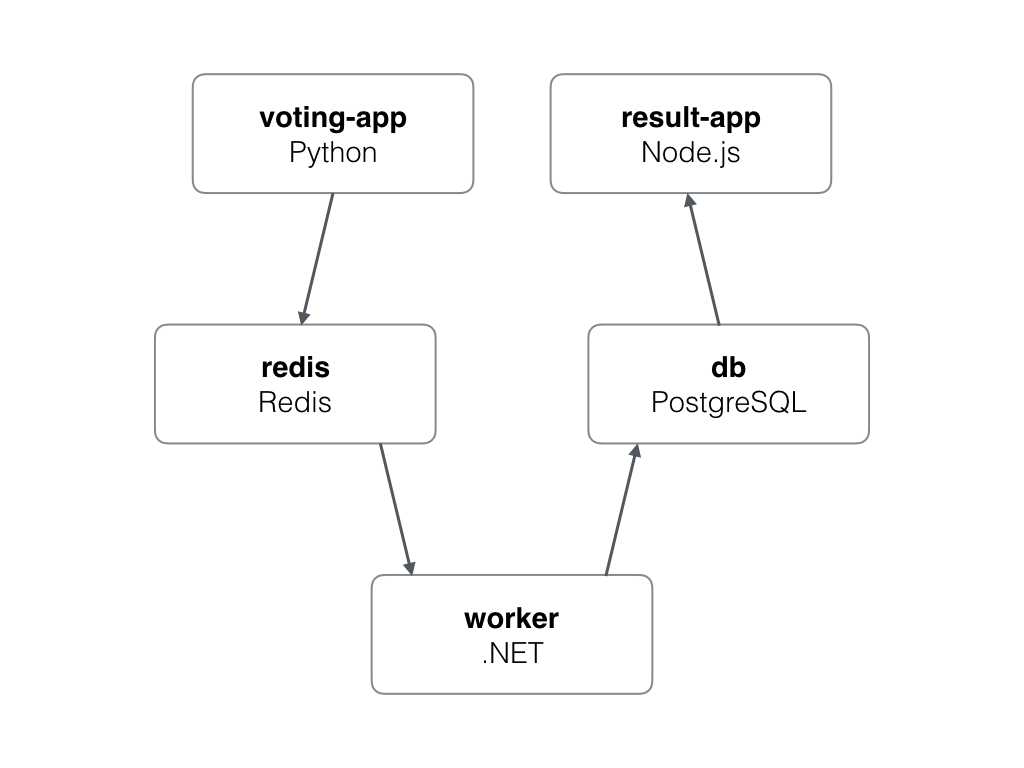
\includegraphics[width=\linewidth]{images/architecture.png}
\label{fig:votingApp}
\end{figure}

It consists of the following components:

\begin{itemize}
    \item A front-end web app
    \item A Redis database collecting new votes
    \item A worker consuming votes and storing them
    \item A Postgres database
    \item A Node.js web app showing the results\footnote{See \textit{Docker (2024)}: Example Voting App. \cite{votingGithub}}
\end{itemize}

After deploying the application, these components will run inside the Kubernetes cluster, each as an individual pod:

\begin{figure}[H]
\centering
\caption {Voting Application Components}
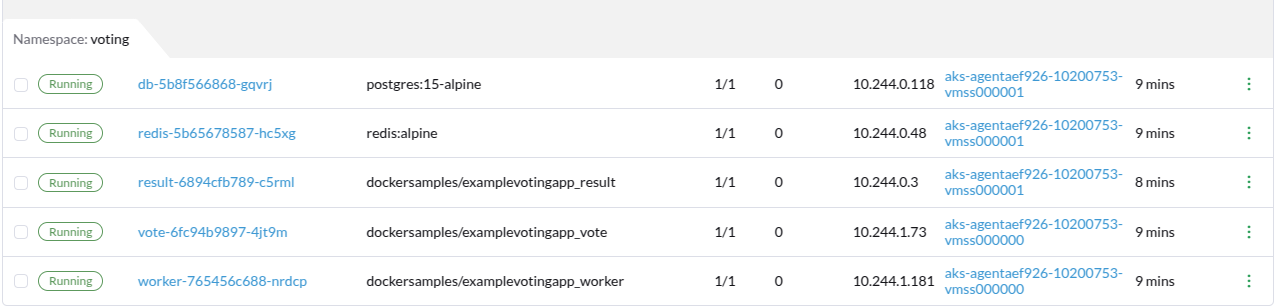
\includegraphics[width=\linewidth]{images/voting-pods.png}
\label{fig:votingPods}
\end{figure}

The YAML files used for the application deployment are on the paper's Github.

Using Rancher's security component Neuvector, we can examine the network connections of the application components:

\begin{figure}[H]
\centering
\caption {Voting Application Connections}
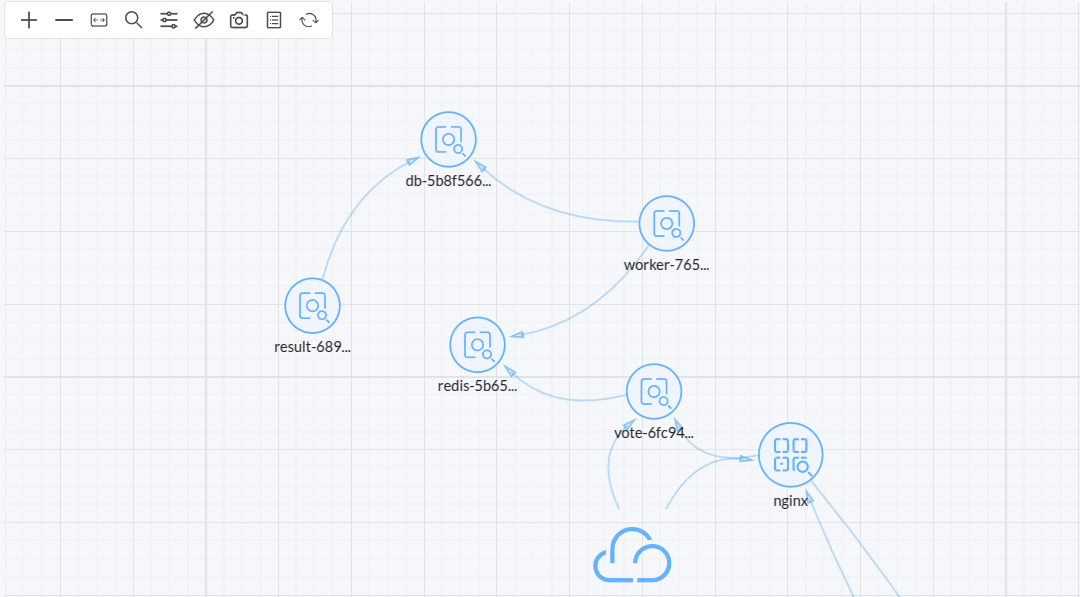
\includegraphics[width=\linewidth]{images/voting-map.png}
\label{fig:votingMap}
\end{figure}

\begin{itemize}
    \item Outside communication will reach the vote front-end, initially through the AKS ingress controller
    \item The vote component will connect to the Redis in-memory database
    \item The worker component will connect to both the Redis and the Postgres database
    \item The result component will read from the Postgres database
\end{itemize}

The arrows indicate the direction in which the connections were established. Without any installed service mesh, all connections are unencrypted. The observed communication relationships match the application documentation.

\subsection{LinkerD}

To install Linkerd, we follow the excellent instructions provided by SUSE.\footnote{See \textit{Dayley, B. (2021)}: End-to-end Encryption with Linkerd. \cite{installLinkerd}}

\subsection{Istio}

